\documentclass[conference]{IEEEtran}
\usepackage{amsmath,amssymb,booktabs,graphicx,balance}
\usepackage[hidelinks]{hyperref}
\hypersetup{pdftitle={Checkpointing Shared Git Events for a Coding Agent's Graph Memory},pdfauthor={Anonymous working draft}}
\usepackage{iftex}
\ifXeTeX
\usepackage{fontspec}
\setmainfont{texgyretermes-regular.otf}[BoldFont=texgyretermes-bold.otf,ItalicFont=texgyretermes-italic.otf,BoldItalicFont=texgyretermes-bolditalic.otf]
\setsansfont{texgyreheros-regular.otf}[BoldFont=texgyreheros-bold.otf,ItalicFont=texgyreheros-italic.otf]
\setmonofont{texgyrecursor-regular.otf}[BoldFont=texgyrecursor-bold.otf]
\fi
\title{Checkpointing Shared Git Events for a Coding Agent's Graph Memory}
\author{\IEEEauthorblockN{Anonymous working draft}}
\begin{document}
\maketitle
\begin{abstract}
A graph memory for coding agents can retain source events shared by multiple files. Reopening an exact SQLite index restores durable evidence, but loses shared events in volatile memory. Our demonstration lets visitors inspect source commits, choose which events to checkpoint and trace the bytes that must be written, restored and fetched. At a fixed 1\,KiB per repository, a checkpoint weighted by historical file participation used 82,907 bytes across 196 subsequent queries, versus 106,186 for recent events and 88,562 for the largest bodies. A complete unpadded snapshot used 69,607 bytes. At 4\,KiB the weighted snapshot used 61,672 bytes. Total execution time did not improve. On six shorter histories all three padded 4\,KiB snapshots cost more than reopening cold. Every policy returned the same top eight paths and scores. Companion scenarios show the different evidence required when one or two files are known and test the limits of transferring these gains to a coding model.

\end{abstract}

\section{Who still holds the evidence?}
A coding agent opens a graph generator and needs to decide which test to read. The generator's latest changes concern utilities used throughout the project. Its test changed with the generator in earlier commits. The generator may have exhausted its retention budget while the less frequently modified test still holds those earlier events. A second question arises when the agent already knows two implementation files. Did a candidate test change with each file on separate occasions, or did all three appear in the same change? A table of pair weights can give the same answer in both situations.

ROSE~\cite{zimmermann} established version histories as a source of file recommendations. Moonen et al.~\cite{moonen} showed empirically that a cutoff on transaction size can improve association-rule recommendations. Higher-order link prediction also distinguishes co-membership in one interaction from the corresponding pair projection~\cite{benson}. Temporal graph systems for agents such as TAPE~\cite{tape} make dated relationships queryable. Our system lets a visitor change the read policy over a fixed event store, inspect the commits added to an answer, and see when the answer can be reconstructed by a smaller representation. Cost-aware caching has long combined retrieval benefit and object size~\cite{cao}. Here one stored event may serve many anchor files. We test how to allocate a small checkpoint using their past participation, with all source data and an exact fallback retained. The visitor can inspect both the saved reads and the cost of writing and reopening that checkpoint.

\begin{figure}[t]
\centering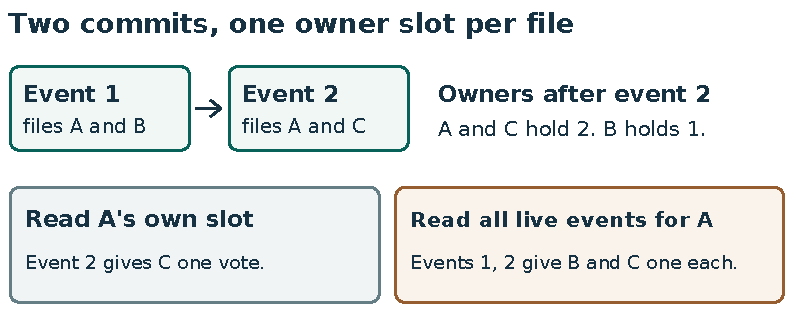
\includegraphics[width=\columnwidth]{retention.pdf}
\caption{After file A evicts its reference to event 1, file B still holds it. The live incidence index points from A to both events.}
\label{fig:retention}
\end{figure}

The Git reader observes paths changed on successive first-parent transitions. It requires no source-content indexing. Each vote can identify a concrete commit, while semantically related files may have no shared change history. The prototype exposes source availability, exact reconstruction and agreement with a subsequent change as separate measurements.

\section{Retention, projection and recovery}
\subsection{Write an event once}
For an accepted Git event $e$, $M_e$ is its set of Python paths and the commit SHA identifies its source. Paths receive integer IDs at their first appearance. Events with 2--64 paths form the co-edit history. Single-file commits can still contribute to recent frequency. Let $O_t(f)$ contain the last $b$ accepted events involving file $f$, with $b=8$. The hot set and the events readable through anchor $a$ are
\[
 H_t=\bigcup_f O_t(f),\qquad I_t(a)=\{e\in H_t:a\in M_e\}.
\]
When a path advances its queue, a released event remains hot as long as another member still owns it. An incidence index identifies all members of a surviving event. One new event with $m$ paths introduces $m$ incidences. Expanding it into directed pair counts would generate $m(m-1)$ updates. The queues, live incidence index and historical archive have separate storage costs.

For a one-file query, each decoded event that contains $a,x$ gives $x$ a vote. The reader may count events, or give each pair weight $1/(|M_e|-1)$ so that one known participant distributes one unit over its partners~\cite{newman}. The ties use file frequency in the preceding 32 commits and then the first-seen ID. An owner-only reader uses $O_t(a)$. A shared reader can use all of $I_t(a)$, or inspect event sizes before choosing which eight bodies to read. Size selection requires access to member-count metadata even when it avoids decoding the bodies themselves.

\subsection{Which exact query can an index answer?}
The exact one-file reader returns the same ordered eight IDs and scores as full co-edit counts. If every event for an anchor is available in cache, its votes can be summed directly. A file with potentially missing history requires the complete list of relevant event IDs. Only missing bodies are fetched. This maintains the same answer after eviction or restart. Approximate recommendations from the retained subset use their own explicit read budget.

For each of two observed files $a,b$, the reader prefers recent surviving events of size at most six and fills up to eight by recency. It takes the union and decodes each event once. For another file $x$, the normalized sum of the pair weights is $p(x)$. A joint event with $a,b,x$ contributes $1/(|M_e|-2)$ to $q(x)$. We compare the rank of $p(x)+q(x)$ with the pair sum alone. A control redistributes the same joint-event mass by the harmonic mean of the two pair weights. It keeps the total joint-event count and discards its candidate-specific assignment. All three rankings share events, candidates and tie rules.

\subsection{Select a checkpoint from retained sources}
A planned restart closes the database after half the accepted events in each repository. Only events in the current hot set are eligible for a snapshot. Let $s_e$ be the encoded member-body size, $c_e$ its cost including the event identifier and length field, and $n_f$ the number of occurrences of file $f$ in the preceding 128 events. Writing $M=M_e$ for its members, we rank eligible events by
\[
     \frac{s_e}{c_e}\sum_{f\in M}(1+n_f).
\]
If future queries name anchor $f$ with mass $p_f$, and each otherwise fetches body $e$ whenever $f\in M_e$, saving $e$ avoids expected transfer $s_e\sum_{f\in M}p_f$ per query. The formula substitutes smoothed prefix counts for the unknown anchor probabilities. Taking high ratios first and skipping entries that exceed the space remaining is a packing heuristic. Posting-list reads, overlapping future cache entries, CPU time and physical page writes fall outside this simple model.

The snapshot includes ordered event IDs and bodies, the source horizon and its SHA. On reopening, the reader validates the horizon, hash and checksum. It pins valid entries for this session. A missing, stale or corrupt snapshot falls back to the complete file index. For a query whose historical coverage is uncertified, the reader loads its posting list and fetches just the bodies absent from memory. A separate live cache handles post-restart events. Equal-budget comparisons store and read exactly the same number of snapshot bytes, with explicit padding. The full snapshot uses its actual length.

\begin{figure*}[t]
\centering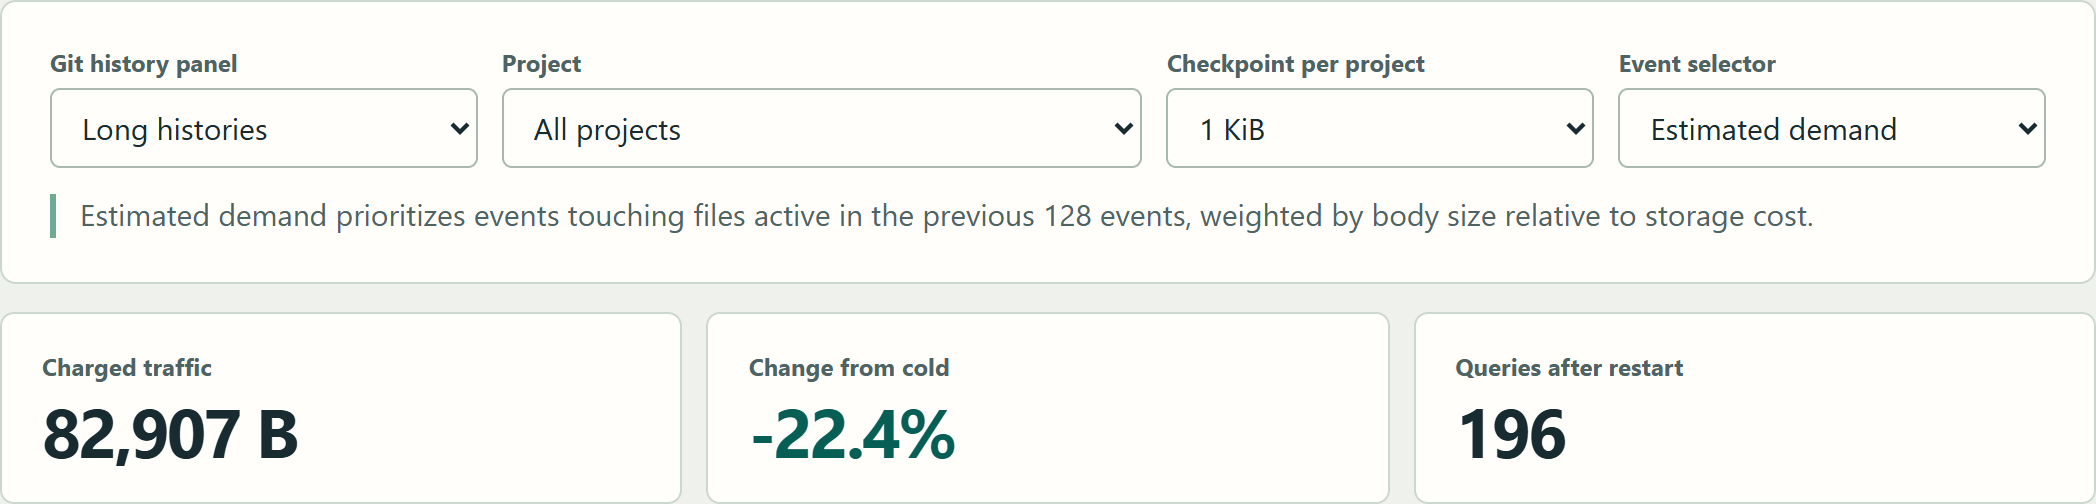
\includegraphics[width=.93\textwidth]{restart-screen.png}
\caption{Checkpoint controls and measurements in the offline console. Switching the selector, budget or repository redraws the cold comparison, the ledger of transferred bytes and end-to-end timing for the same recorded workload.}
\label{fig:restart}
\end{figure*}

\section{Visitor scenarios}
\subsection{Track the lifetime of a test's evidence}
Open the NetworkX directed-generator case. In the owner-only view, eight events contain 252 file memberships. In the shared view, 15 events contain 421 memberships. Four additional commits move the actual test to rank five with six votes. Expanding \texttt{539ad536} shows that the test retained a source already evicted by the generator. For the HITS implementation before \texttt{1e5933df}, sharing instead adds two votes to a test previously ranked fourth. Competing files gain even more and the test drops outside the eight suggestions. Visitors can inspect all 15 additional events and follow their links to Git.

\subsection{Give the agent two known files}
Open \texttt{seed\_pair/demo.html} offline, or run \texttt{demo.py serve} in its directory and choose the live SQLite source. The console lets a visitor choose a real commit, inspect the two revealed paths and compare distinct uses of the same source records. Before Dask commit \texttt{06c1bb72} in the SQL replay, the known paths are the array package initializer and its expression module \texttt{\_io.py}. Of the three held-out paths, the pair sum finds zero, candidate-specific joint evidence finds two, and redistributing the same joint mass by harmonic pair support finds all three. For xarray commit \texttt{503b262d}, the pair sum recovers one of two targets while the joint score recovers neither. Visitors can inspect the history rows that support each candidate, then reveal the reference targets to annotate the predicted order.

Switch from a real commit to two constructed histories (Fig.~\ref{fig:pair}). For three groups $A,B,C$ each of size $n$, history $s$ consists of events $(A_i,B_j,C_{(i+j+s)\bmod n})$. Every cross-group pair appears once for every $s$. The visitor may compare pair counts across histories before opening the event for $(A_i,B_j)$. A change of $s$ changes its third file while every pair count is preserved. Across uniformly weighted histories any method with only these pair counts has expected Hit@$k\le k/n$ for $k\le n$. The $n=16$ replay has 768 equal pair counts across worlds, 256 queries per world and 4,096 in total. At $k=8$ the pair-only ceiling is 2,048 hits; preserved events identify all 4,096 third members. File-pair timestamps or event identifiers may retain the missing information and fall outside that bound.

\begin{figure}[t]
\centering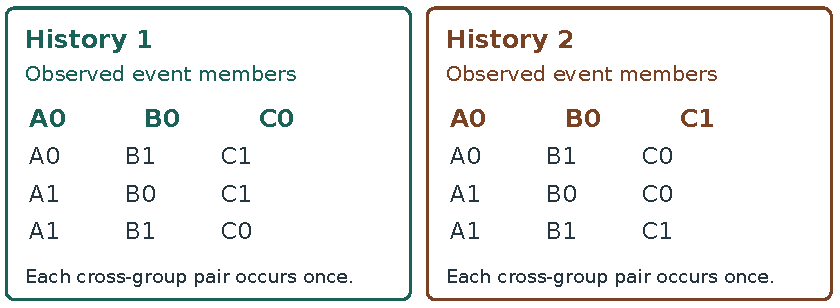
\includegraphics[width=\columnwidth]{pair-worlds.pdf}
\caption{Two possible histories, shown at $n=2$. The bold rows give different third members for the same known files. Every individual pair of files across the three groups has the same count in the two histories.}
\label{fig:pair}
\end{figure}

\subsection{Choose what survives a restart}
Open the checkpoint console (Fig.~\ref{fig:restart}) and start with the long-history panel. Select the 1\,KiB budget and switch between recent events, the largest bodies and estimated demand. Each comparison reports the same exact ranked answers. The ledger separates snapshot write and load bytes, validation receipts, the posting lists read through SQLite and the bodies missing from the recovered cache. The project selector shows which histories account for an aggregate difference. The timing table includes the entire write--restart--read sequence.

Choose the short-history panel and select the 4\,KiB budget. The interface can also jump to this reversal with the \emph{Show a cost increase} button. The useful contents and padded length explain the result. Select the unpadded full snapshot to see how many bytes are needed when every retained event fits. At the adjacent editor-cache tab a visitor can choose a real recorded SWE-agent window and see how many previously viewed bytes fit under a fixed serialized capacity. Both tabs replay observations from actual executions. The earlier SQL console additionally supports interactive queries against the event database.

\section{Measured costs and predictive utility}
\subsection{Replicating one-file selection}
We predict companion paths from the Git prefix before inserting a held-out multi-file commit. Recall@8 counts its other paths among eight suggestions, including previously unseen targets in the denominator.

\begin{table}[t]
\caption{Independent one-anchor panel. Both ranking weights and size thresholds were held fixed before evaluating 932 queries. Macro recall gives each project equal weight. The byte count measures decoded member IDs.}
\label{tab:replication}\centering\small
\setlength{\tabcolsep}{3.5pt}
\begin{tabular}{@{}lrrrr@{}}\toprule
Weighted read & Macro R@8 & Pooled R@8 & Events & Bytes \\\midrule
Last eight & 58.39\% & 61.76\% & 5,953 & 280,888\\
Size $\le6$, then fill & 58.72\% & 62.58\% & 5,953 & 187,864\\
Strict size $\le6$ & 59.45\% & 62.56\% & 4,737 & 60,196\\
Strict size $\le8$ & 59.29\% & 63.24\% & 5,060 & 73,524\\\bottomrule
\end{tabular}
\end{table}

On six new repositories, 932 one-anchor queries tested the frozen size rule (Table~\ref{tab:replication}). Both main arms give each pair the same inverse-size weight. The challenge arm prioritizes the newest available events containing at most six paths, filling any remaining slots by recency. The control reads the anchor's last eight. Across identical numbers of decoded events the new rule reduced decoded member bytes by 33.1\%. The mean project-level recall difference was $+0.33$ points, paired 95\% bootstrap interval $[-0.57,+1.43]$ across six projects. Per query there were 44 wins, 54 losses and 834 ties. The literal size cutoffs adapted from Moonen et al. were competitive and read substantially fewer bodies. The modeled bytes exclude metadata discovery, queue maintenance and the cost of applying the policy.

\subsection{Charging the checkpoint and its subsequent reads}
The durable baseline stores each event's full binary SHA and ordered variable-length file IDs, plus complete chronological postings per file. Inserts use a SQLite WAL transaction with synchronous mode FULL. The three long histories occupy 323,584 bytes after WAL checkpoint and truncation, excluding common path dictionaries and tie metadata. Sharing volatile events on these same files served 196 exact warm queries in 21,142 bytes versus 123,058 for owner-only caching. After losing the shared cache midway, all 196 queries fell beyond the boundary and required 106,781 bytes. This motivates paying for optional state at a planned restart.

\begin{table}[t]
\caption{Measured application bytes, summed over projects. Both snapshot directions, a 20-byte source receipt per reopened snapshot, subsequent postings and missing event bodies are charged. Fixed budgets apply per project. The complete snapshot has no padding.}
\label{tab:storage}\centering\small
\setlength{\tabcolsep}{3.5pt}
\begin{tabular}{@{}lrr@{}}\toprule
Checkpoint & Long (196 queries) & Short (492 queries) \\\midrule
Cold & 106,781 & 34,309\\
Recent, 1\,KiB & 106,186 & 19,358\\
Largest bodies, 1\,KiB & 88,562 & 18,105\\
Historical demand, 1\,KiB & 82,907 & 18,063\\
Recent, 4\,KiB & 93,263 & 53,808\\
Largest bodies, 4\,KiB & 62,827 & 53,808\\
Historical demand, 4\,KiB & 61,672 & 53,808\\
Complete, unpadded & 69,607 & 12,168\\\bottomrule
\end{tabular}
\end{table}

We ran eight policies over nine repositories in three randomized orders. All 25,824 comparisons of ordered IDs and scores agreed with complete reconstruction, including 16,512 after the restart. Timing repeats are not independent projects. Reconstructing the byte ledger separately from input events confirmed each post-restart query. Missing, corrupt and outdated snapshots also preserved the correct answers in the tested fault paths.

On the three long histories (Table~\ref{tab:storage}), estimated demand saved 21.9\% against recency at 1\,KiB. Choosing long bodies alone captured most of this saving. The additional reduction relative to that control was 6.4\% at 1\,KiB and 1.8\% at 4\,KiB. The 1\,KiB method needed 19.1\% more application bytes than a complete snapshot on this panel. At 4\,KiB it used 11.4\% fewer. On the short panel complete snapshots gave the lowest observed traffic. Suppressing padding in the short 4\,KiB sensitivity yields the same 12,168 bytes. With actual 1\,KiB snapshots the long panel added 12,288 bytes of database footprint and generated 24,816 WAL bytes at the checkpoint. The application-byte metric measures a different boundary. With the realized future requests, the lower and upper bounds of an offline packing calculation both gave 33,439 as the maximum archive bytes saved at 1\,KiB on the long panel. Historical demand saved 30,078, all in event bodies. This bound excludes the fixed cost of checkpoint transfer.

The median aggregate post-restart query time on the long panel was 38.62\,ms cold, 38.07\,ms with the recent 1\,KiB snapshot, 36.91\,ms for largest bodies, 35.82\,ms for estimated demand and 27.69\,ms for the full snapshot. Corresponding medians for the entire instrumented stream were 2.400, 2.388, 2.404, 2.407 and 2.381\,s. Improved transfer did not yield a measured full-run speedup. The experiment uses a single writer and a planned checkpoint.

We froze the policy and evaluated 12 additional repositories. Under sparse queries, the 1\,KiB demand snapshot charged 37,640 bytes for 189 post-restart requests, versus 42,103 for recency and 37,944 for size. Cold opening required only 30,987 bytes and beat the demand policy on nine projects. Under dense requests (2,063), demand used 151,189 bytes versus 202,250 for recency and 335,947 cold. An unpadded full snapshot used 131,923. The archive graded 32,632 exact outputs in 192 SQLite runs over both schedules. A further control wrote and reopened the shorter SQLite snapshots without padding, then reused the query trace after verifying identical recovered states. Under sparse demand, the 1\,KiB demand, recent and size policies then used 32,566, 37,031 and 32,878 bytes. Cold still required only 30,987. Under dense reads unpadded demand cost 146,115 versus 131,923 for full restoration. The ability to amortize checkpoint transfer depends on how often the session reads the archive.

\balance
\subsection{Which improvements reach a coding agent?}
On an independent two-anchor panel, 621 queries from six additional repositories yielded pooled Recall@8 of 36.89\% for the pair sum, 37.19\% for candidate-specific joint votes and 37.82\% for the mass-matched harmonic control. A joint event was available in 314 queries. The joint-versus-sum change averaged $+0.17$ points by repository with interval $[-1.17,+1.42]$. The mathematical construction establishes what pair counts can lose. The controlled real data leave the quality benefit of storing candidate-specific three-way evidence unresolved.

On Agent Retrieval Bench~\cite{arb}, seven published rankings were reproduced on 106 code-to-test tasks. Adding one history-based suggestion to role-filtered Qwen3-Embedding-4B on a 105-task panel changed Recall@5 from 68.98\% to 69.62\% (paired difference interval $[-2.58,+3.30]$ points).

We also tested a solver decision on 21 held-out functions from three Python libraries. A local Qwen3-4B-Instruct-2507 drafted a function with one historical test. A tool exercised up to six earlier assertions on the draft. An independent model call received either the first BM25-ranked assertion and its status, the highest-ranked failed assertion with its status, that same assertion with its status hidden, or no new evidence. Each review had the same input budget. Across 87 new greedy generations the two status-visible alternatives each passed all original doctests on 7/21 functions and 46/85 individual examples. Choosing a failure changed the retrieved record for three functions and the implementation for one. The other two controls each solved 8/21 functions. In a companion replay of 108 archived SWE-agent~\cite{sweagent} sessions, sharing identical line bodies across addresses at 16\,KiB with fixed-width addresses served 273,243 previously seen bytes versus 257,099 across 822 views. In a compact encoding, sharing across files added 4,978 served bytes beyond within-file deduplication, with 60 complete windows under both policies. These replays preserve the recorded action sequence. Whether agent task completion benefits from checkpointing remains open.

\section*{Acknowledgments}
OpenAI Codex drafted and revised the paper, implemented and exercised the prototypes, and analyzed the archived outputs. The replication materials include the frozen policies, per-query decisions and checks against independently reconstructed histories.

\bibliographystyle{IEEEtran}
\bibliography{sources}
\end{document}
